\beginsong{Ziehharmonika}[txt={Theodor Kramer}, mel={Singekreis Silberburg, Karlsruhe}, index={Nicht für's Süße, nur für's Scharfe}, siru={172}, biest={612}]

% \beginverse
% \[Am]Nicht für's \[F]Süße, \[C]nur für's \[G]Scharfe \[Am]und für's \[F]Bitt're \[C]bin ich \[G]da,
% \[C]schlag, ihr \[E]Leute, \[Am]nicht die Harfe, \[F]spiel' die \[G]Ziehhar\[Em]moni\[Am]ka.
% \[Am]Lai la \[F]lai lai, \[G]lai la \[C]lai lai, \[Am]lai la \[F]lai lai,\[G] lai la \[Am]la,
% \[F]Schlag, ihr \[G]Leute, \[Am]nicht die Harfe, \[F]spiel die \[G]Ziehhar\[Em]moni\[Am]ka.
% \endverse

\beginverse
\endverse
\centering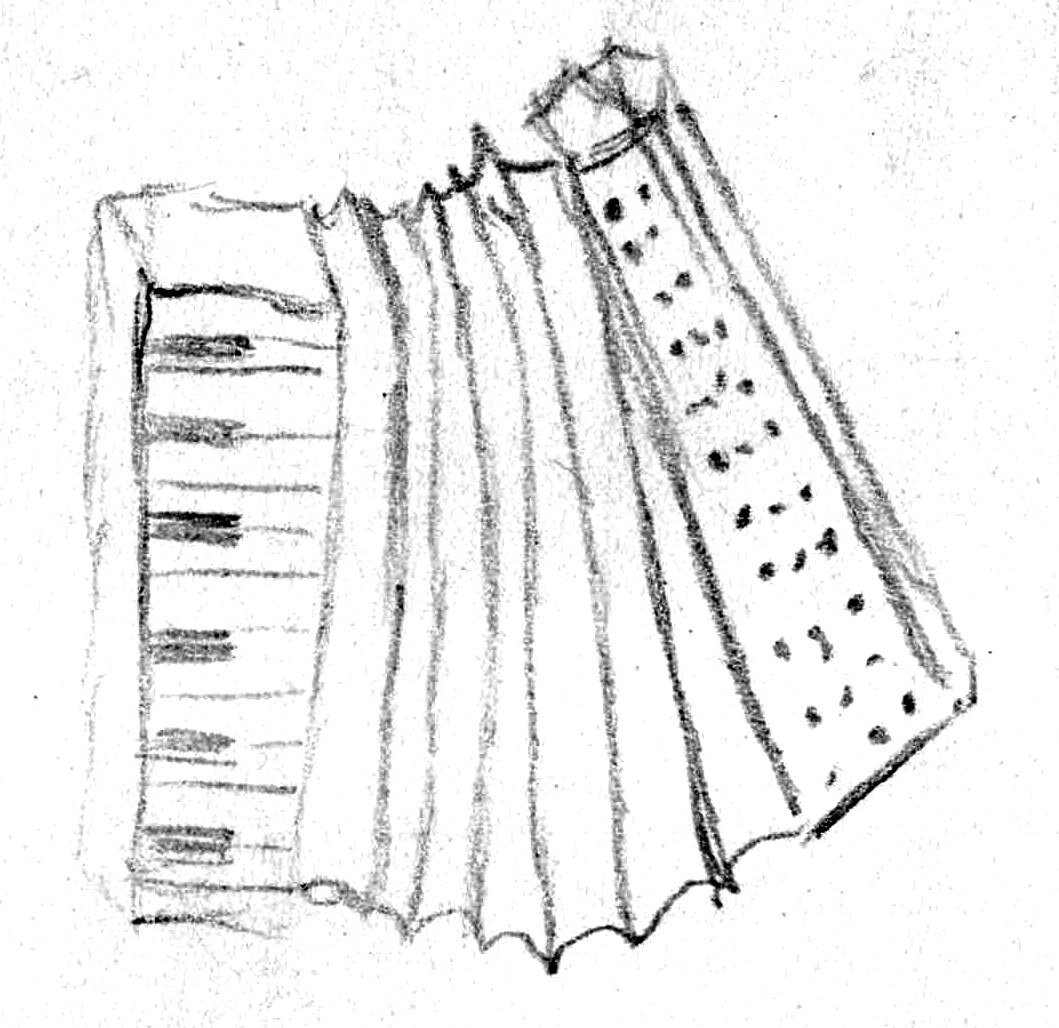
\includegraphics[width=1\textwidth]{Noten/Zieharmonika.pdf}

\beginverse
\[Am]Leer, ver\[F]filzt ist \[C]meine \[G]Tasche \[Am]und durch\[F]löchert \[C]ist der \[G]Hut,
\[C]dass ich \[E]leb', das \[Am]Herz aus Asche, \[F]macht: Aus \[G]Branntwein \[Em]ist mein \[Am]Blut.
\[Am]Lai la \[F]lai lai, \[G]lai la \[C]lai lai, \[Am]lai la \[F]lai lai,\[G] lai la \[Am]la,
\[F]dass ich \[G]leb', das \[Am]Herz aus Asche, \[F]macht: Aus \[G]Branntwein \[Em]ist mein \[Am]Blut.
\endverse

\beginverse
^Ließ' das ^Salz der ^Tränen ^Spuren, ^wären ^meine ^Gucker ^blind,
^meine ^Liebsten ^sind die Huren, ^mir Ge^sellen ^Staub und ^Wind.
^Lai la ^lai lai, ^lai la ^lai lai, ^lai la ^lai lai,^ lai la ^la,
^meine ^Liebsten ^sind die Huren, ^mir Ge^sellen ^Staub und ^Wind.
\endverse

\beginverse
^Das Fal^sett, das ^möcht' um^armen, ^doch das ^Ganze ^trägt der ^Bass,
^hab' Er^barmen, ^brauch' Erbarmen, ^doch zu^innerst ^haust der ^Hass.
^Lai la ^lai lai, ^lai la ^lai lai, ^lai la ^lai lai,^ lai la ^la,
^hab' Er^barmen, ^brauch' Erbarmen, ^doch zu^innerst ^haust der ^Hass.
\endverse

\beginverse
^Weiß zu ^viel und ^möcht' doch ^träumen ^wie der ^Echs im ^Sonnen^schein,
^leeres ^Brausen ^in den Bäumen, ^braus' für ^mich, nick' ^träg' ich ^ein!
^Lai la ^lai lai, ^lai la ^lai lai, ^lai la ^lai lai,^ lai la ^la,
^leeres ^Brausen ^in den Bäumen, ^braus' für ^mich, nick' ^träg' ich ^ein!
\endverse

\beginverse
^Darf nicht ^ruh‘n, muss ^Straßen ^weiter; ^denn bald ^bin ich ^nicht mehr ^da.
^Und es ^spielt die ^Stadt kein zweiter ^so die ^Ziehhar^moni^ka.
^Lai la ^lai lai, ^lai la ^lai lai, ^lai la ^lai lai,^ lai la ^la,
^Und es ^spielt die ^Stadt kein zweiter ^so die ^Ziehhar^moni^ka.
\endverse

\endsong

\begin{intersong}
\ifthenelse{\boolean{pics}}{
    \ThisLRCornerWallPaper{0.40}{Bilder/Zieharmonika.png}
}{}
\end{intersong}